% uncomment the desired options
\documentclass[%
        %draft,
        %submission,
        compressed,
        %final,
        %
        %technote,
        %internal,
        %submitted,
        %inpress,
        %reprint,
        %
        %titlepage,
        notitlepage,
        %anonymous,
        narroweqnarray,
        inline,
        %twoside,
        ]{ieee}

% the next line uses Postscript fonts instead of the Computer Modern ones
%\usepackage{times}

\begin{document}

\title[Game Playing With Genetic Algorithms]{Game Playing With Genetic Algorithms}

\author[LAU, ODORJAN, VOINO]{
      Edmond Lau
    \and
      Chris Odorjan
    \and
      Richard Voino
  }

\date{April 9, 2002}

\maketitle               

\begin{abstract}
\it{
Genetic algorithms are powerful means for solving many types of artificial
intelligence problems. They bring many methods used by nature to evolve
creatures suitable for their environment into the realm of computer
learning. This paper describes a simple game resembling hockey or soccer
that can be used to test the feasibility of a genetic algorithm to adapt
rule-based agents to their environment using computer-based learning.
}
\end{abstract}

\section{Introduction}

\PARstart Genetic algorithms are simple and easily-implemented methods of
reinforced computer learning. The language of genetic algorithms is similar
to biological genetics, and terms from both fields are used interchangeably
in this paper.

A genetic algorithm evolves individuals based upon their suitability, or
fitness to their environment. Organisms that perform poorly in their
environment die off, while organisms that perform well live long enough to
reproduce. This ensures that genomes that have shown to be somewhat
successful in the past are propagated to new organisms, while genomes that
are unsuccessful are removed from the system.

This paper describes an implementation of a genetic algorithm and a simple
game to test the suitability of this genetic algorithm for reinforced
learning.

\section{The Game}

To test the implementation of a simple genetic algorithm a game similar to
hockey and soccer was devised.

\subsection{Game Definition}

The game is played in an arena twice as wide as it is high, with the
ball initially placed in the centre and two nets at either end. Two teams
with any number of players are lined up, one team on each side of a line through the
centre of the arena. The players are evenly spaced before the game begins.

When the game begins, players may move in any direction. If a player comes
in contact with the ball, it takes possession of it. The player may then
carry the ball along with itself, pass the ball to another player, or shoot
the ball at the net. If a player with the ball comes in contact with a
player on the opposing team, there is a chance that the other player can
take possession of the ball.

Goals are scored when the ball enters the net, either by being carried by a
player, or if it is shot into the net by a player. The team that the player
is on receives a positive goal if the ball entered the opposing team's net,
or a negative goal if the ball entered their own net. After a goal is
scored, players move back to their positions as before the start of the
game, and the ball is again placed at the centre of the arena. Then the
gameplay resumes.

The game continues for a predefined amount of time. At the end the score is
tallied; if the scores are equal then both teams receive a tie, otherwise
the winning team receives a win and the losing team receives a loss.

\subsection{Assumptions}

Since shooting and passing the ball are the same operation, this
implementation defines them as ``firing'' the ball.

Players are defined by Bots. Each bot is given a mass; more massive
bots can fire the ball faster, but they themselves move more slowly.

All movement for both bots and the ball is defined in terms of a ``tick.''
The speed of the object determines how many ticks it takes before the object
is given a turn to move. Bots may move, rotate, or fire the ball
if they have it on each turn, but cannot perform more than one of these
operations per turn.

After each goal the positions of each bot and the ball are reset, and
gameplay resumes. When a predefined number of ticks have been processed the
game ends. Currently a game ends after 1000 ticks; when this occurs, the
play stops and a simple genetic algorithm is performed on each team
separately.

\section{Genetic Algorithm}

The main aspects of the simple genetic algorithm in this implementation are:
\nopagebreak
\begin{description}
\item[Bot Fitness:] determines survival and suitability for reproduction
\item[Crossover Function:] evaluates bot performance and ``mates'' them
\item[Mutation:] occasionally randomizes bot rules
\end{description}

\subsection{Bot Fitness}

The fitness of each bot is measured by its performance during a game.
Currently, goals scored are weighed the highest, followed by interceptions
made and time with the ball. These scores are summed using the following
function, where $G$ represents goals scored by the bot, $I$ is the number of
interceptions made by the bot, and $T$ is the number of ticks that the bot
had possession of the ball for. $W_{G}$, $W_{I}$, and $W_{T}$ are the
weights of the three scores, respectively.
\begin{displaymath}
W_{G} * G + W_{I} * I + W_{T} * T
\end{displaymath}
The result of this function is the fitness of the bot. Since goals scored
can be negative, so can the fitness.

The weights are currently set to:
\nopagebreak
\begin{description}
\item[goals:] 1.0
\item[interceptions:] 0.5
\item[time with the ball:] 0.2
\end{description}

\subsection{Crossover Function}

After each game, the fitness function is computed for each bot and the bots
are sorted by their fitness. The number of bots to replace on the team is
half of the size of the team, rounded down to the next lowest even integer.
The lowest scoring bots are removed from the team, and the highest scoring
bots are used as input to the crossover function. The crossover function
takes a random number of rules from the first parent bot and a
different random number of rules from the second parent bot to form one child
bot. A second child bot is formed from the remaining rules. These new bots
are used to replace the bots that were removed from the team.

\subsection{Mutation}

After the new team has been generated, each bot on the team has a small
chance of being mutated. When this occurs, one of the rules of the chosen bot is
mutated; that is, one element of the rule is changed.

\section{Rules}

\subsection{Rule Sets}

Each bot stores a number of rules, consisting of six different elements.

Three of the elements are conditions:
\nopagebreak
\begin{description}
\item[sensor array (of eight elements):] indicates an object (or nothing)
within the sensor range of the 8 cardinal directions of the bot 
\item[teamBall:] an integer that is negative when the opposing team has the
ball, positive when the bot's own team has the ball, and zero if the ball is
free
\item[myBall:] true when the bot itself is in possession of the ball
\end{description}

The three remaining elements are actions:
\nopagebreak
\begin{description}
\item[fire:] indicates that the bot should fire the ball when the conditions are met 
\item[move:] indicates that the bot should move one space in the direction it is facing 
\item[turn:] one of Left, Right, or None, indicating a direction for the bot to turn to
\end{description}

The structure of each rule is summarized in Fig.~\ref{fig:rule}.

\begin{figure}[htp]
\centering
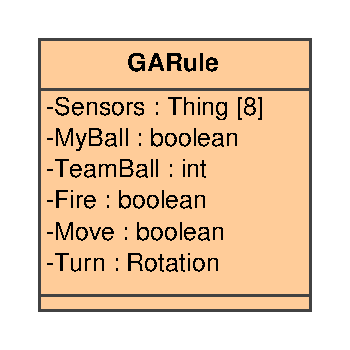
\includegraphics[width=0.3\textwidth]{rule.eps}
\caption[GARule]{GARule Structure}
\label{fig:rule}
\end{figure}

\subsection{Rule Evaluation}

When a bot is given the chance to move, it determines its own state. This
state is then programmed into the conditions of a new rule, which is
compared to each of the bot's own rules using a function that returns a
non-negative integer representing how closely the given conditions match the
rule. If the function returns a zero, then the conditions of the two
rules are the same. The results of applying the function to each rule are sorted
in ascending order, so the closest matching rule is first. If more than one
rule matches, then one of these is executed at random, otherwise the matching
rule is executed.

\subsection{Rule Execution}

Rule execution consists of performing one of the actions specified
in the rule. Only one action may be performed, so if the rule specifies
more than one action, the following preference is given:\nopagebreak
\begin{enumerate}
\item fire 
\item move 
\item turn 
\end{enumerate}

Movement also involves checking if the bot collided with another bot,
a wall, or the ball. When two bots collide, they both turn away from
each other in the hopes that they do not collide again upon their next
turn, which would prevent either bot from moving.

Bot collisions with walls have no effect; the bot stays in the position it
was in before executing the rule.

When the bot collides with the ball, it takes possession of the ball and may
carry it or fire it on its next turn. If a bot is in possession of the ball, then
the ball moves along with the bot when the rule is executed.

\section{Implementation}

The described system is implemented entirely in C++. The Qt Toolkit is used
for the graphical user interface. This toolkit provides built-in templates
for doubly-linked lists and sortable arrays that are used in the
implementation. It also provides an XML parser that is used for storage of
data.

A copy of the entire code is presented in the Appendix.

\subsection{Implementation Structure}

The implementation of this software package consists of the
following 14 classes:
\nopagebreak
\begin{description}
\item [Arena:] responsible for display of the arena
\item [Ball:] describes and performs operations on the ball in the game
\item [Bot:] describes a bot, provides storage for its rule set, and
provides operations on them
\item [Botview:] responsible for display of objects
\item [Coordinate:] storage for two-dimensional Cartesian coordinates
\item [GABot:] main data storage class
\item [Game:] performs the actual game play
\item [GARule:] describes a rule
\item [MainWindow:] display of the main window
\item [Random:] static class to encapsulate some useful random number
generation functions
\item [SimpleGA:] performs genetic algorithm evolution operations on a team
\item [Team:] describes a team, provides storage for the bots on it, and
provides operations on them
\item [TeamData:] responsible for loading and saving bot data to XML files
\item [TeamParser:] handler for parsing an XML file when loading team data
\end{description}

There are also three enumerated types defined: 
\nopagebreak
\begin{description}
\item [Direction:] cardinal directions (N, NE, E, SE, S, SW, W, NW) 
\item [Rotation:] turn directions (Left, Right, or None) 
\item [Thing:] things that may be perceived by bots (other bots, walls, the ball, nets)
\end{description}

\subsection{Data Storage}

Team data can be saved at any point during gameplay. The data is saved in a
simple XML format to allow easy parsing by the Qt Toolkit's XML parser, and
allows the data to be read by humans. An example team data file is in the
Appendix.

\subsection{Development}

The system was developed entirely on x86-type processors running Linux, but
it has been compiled and runs on Windows, and likely runs on any system that Qt has
been ported to.

Versions 2.2.4, 2.3.2, and 3.0.2 of the Qt toolkit were used and tested during development.
The software compiles using GCC versions 2.95 and 2.96, and Visual C++ 6.0.

\subsection{Screenshots}

Fig.~\ref{fig:filemenu} is a screenshot of the file menu.

Fig.~\ref{fig:gameplay} and Fig.~\ref{fig:game2} are screenshots of the main
window while a game is being played. There are five bots on each team in
both cases.

\begin{figure}[htp]
\centering
\includegraphics[totalheight=0.25\textheight]{screenshots/screenshot_filemenu.eps}
\caption[File Menu]{File Menu}
\label{fig:filemenu}
\end{figure}
\begin{figure}[htp]
\centering
\includegraphics[width=0.8\textwidth]{screenshots/screenshot_play.eps}
\caption[Gameplay 1]{Playing the Game}
\label{fig:gameplay}
\end{figure}
\begin{figure}[htp]
\centering
\includegraphics[width=0.8\textwidth]{screenshots/screenshot_play2.eps}
\caption[Gameplay 2]{Playing the Game}
\label{fig:game2}
\end{figure}

\section{Experiments}

Most of the experiments were performed using randomly-generated teams, known
as ``Team Stochastic'' to reflect their random nature. As the rules for Team
Stochastic are randomly generated, many of them do not make sense in the
context of the game. \nopagebreak Some of the problems are:
\begin{itemize}
\item Specifying multiple actions is redundant, as only one
will be performed.
\item Mutation can produce rules that are never used. For example, the
random rule generating method does not specify ``myBall'' when ``teamBall''
is not positive, but mutation may change this.
\item Some combinations of conditions are not possible; for example, ball
can appear in more than one sensor direction even though there is only one
ball during gameplay.
\end{itemize}

The default team size is five, so one bot on each team is placed directly
in front of the ball. In most games, these bots move directly towards
the ball and the bot who gets there first (generally the bot with the
smaller mass) acquires control of the ball and either fires or carries it
into the net. Because of this games are usually one-sided, but sometimes
(due to random execution of multiple matching rules) the losing team can
still score. As a result of scoring, these bots continue on to the next
generation in the next game. After a short number of games, all of the bots
have more-or-less identical rulesets and run towards the net with the
ball or fire it immediately. The respective speeds of the central bots determine
which team will win.

After many generations, evolved teams were played against newly-generated
teams. The bots on the random teams performed almost as well as evolved
bots, and many times they performed better.

\section{Conclusions}

There are many assumptions and simplifications made in the current version
of this implementation that should be explored further to determine their
effect on learning of the game. Some of the more important ones with
possible solutions are described below.

The total number of possible rules (including rules that contradict
themselves or do not make sense in the context of the game) is
$6^8 \times 3 \times 2 \times 2 \times 2 \times 2 \times 3 = 120932352$.
Randomly-generated bots only contain 100--200 rules, so it is likely that
most of the generated rules do not make sense. The random rule generating
function could analyse the rules, and return only those that can be used by
bots.

Bots that have possession of the ball, even if they are not moving, will
receive a high value of the fitness function. Making $W_T$ smaller, possibly by a
factor of 10 or more can reduce bots that fail to score goals or make
interceptions but achieve a high value of the fitness function and therefore
continue to the next generation.

Collisions with the wall should be added to the fitness function, with a
negative weight. In many test runs bots would simply run towards the wall
and stay there.

The crossover function always replaces bots, so bots that have performed
well in the past can be removed if they play one poor game. The crossover
function used in this simple genetic algorithm produces a team of similar
bots, causing each game to be played in the same way when the same rules get
used again and again.

Unused and duplicate rules can exist in a bot, and some means should be
provided to remove these entries to allow faster matching of rules to
conditions. A counter that is incremented every time a rule is used can be
used to eliminate unused rules, and duplicate rules can be removed after the
crossover function and mutation are completed.

Mutation needs to be explored further, as it can be used to prevent teams
from ``stagnating,'' or having all bots nearly identical.

The implementation of the game and genetic algorithm shows that a genetic
algorithm, even a very simple one, can be used by a computer to learn how to
play a simple game. Although a genetic algorithm can be very powerful, there
are some simplifications made in this implementation that should be
expanded on in future versions.

\bibliographystyle{IEEEbib}
\begin{thebibliography}{1}
\bibitem{key-2}Dalheimer, M., Programming with Qt, O'Reilly, 1999
\bibitem{key-1}Norvig, P., Russell, S., Artificial Intelligence A Modern Approach,
Prentice Hall, 1995
\bibitem{key-3}Stroustrup, B., The C++ Programming Language, Special Edition (3rd),
Addison Wesley, 2000\end{thebibliography}

\end{document}
